Alle im Folgendem beschriebenen Eingaben sind ausschließlich für den Super User sichtbar und können auch nur von ihm durchgeführt werden. Um zu diesen Eingaben zu gelangen muss im Data-Input Menü auf Administration geklickt werden. Im anschließend erscheinendem Menü stehen die nun folgenden Eingaben zur Auswahl zur Verfügung. (siehe \autoref{fig:instr_other_menu})
\begin{figure}[H]
\centering
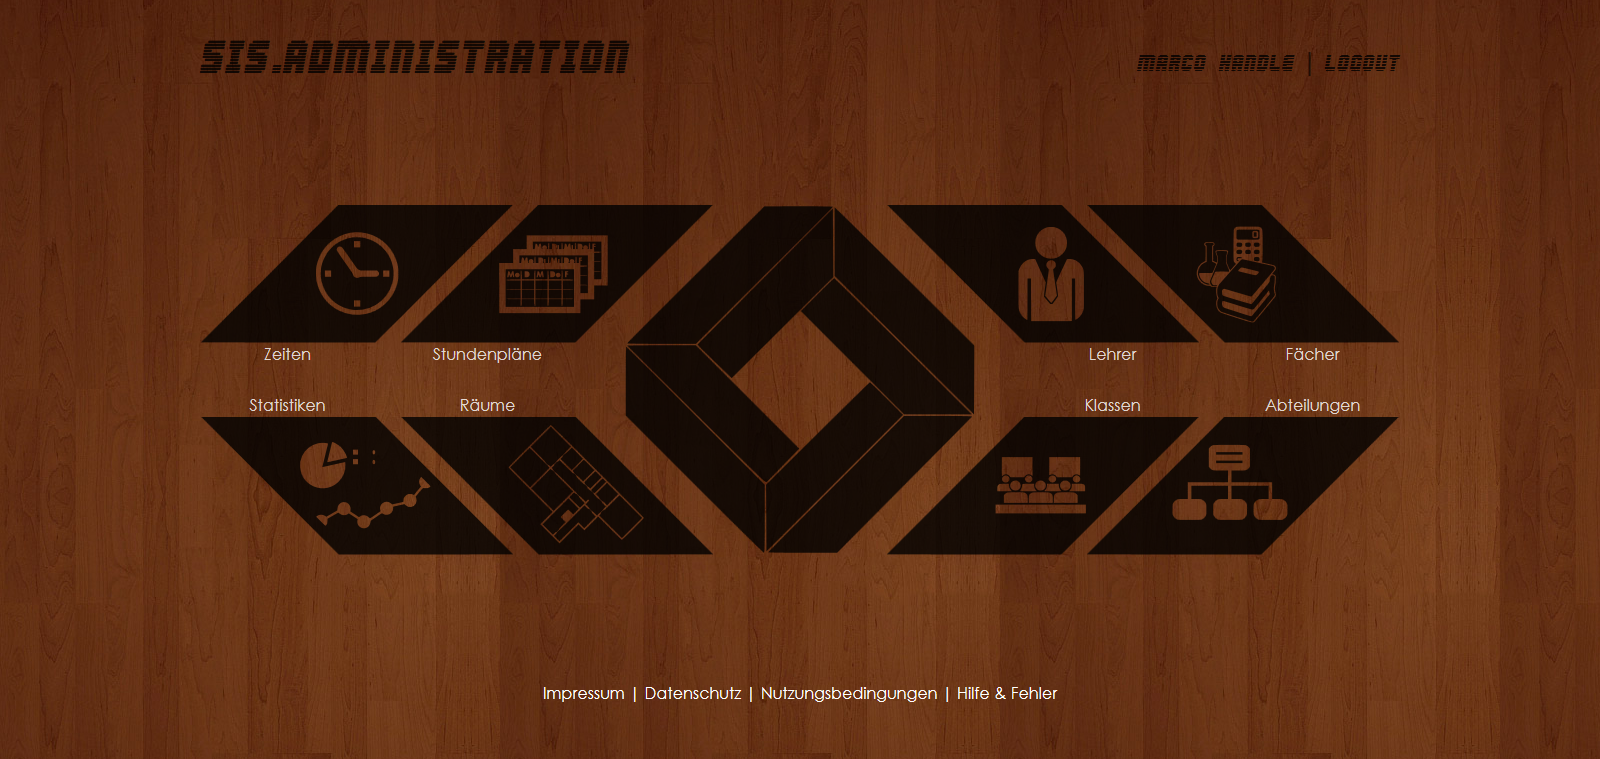
\includegraphics[keepaspectratio=true, width=17cm]{images/screenshots/admin_menu.png}
\caption{Administrationsmenü}
\label{fig:instr_other_menu}
\end{figure}
\subsection{Stunden}
Sollte es aus irgendeinem Grund dazu kommen, dass es mehr Stunden gibt oder sich die Start- und End-Zeiten der Stunden ändern kann dies hier vorgenommen werden.\\
Aus Sicherheitsgründen können Stunden nicht gelöscht werden, da es bei unabsichtlichem Löschen dazu kommt, dass die ganze Stundenpläne und Supplierpläne nicht mehr funktionieren. Deshalb eben diese Sicherheitsmaßnahme.\\
Die Eingabe ist so aufgebaut, dass man mit den Buttons rechts und links den Wochentag auswählen kann. Hat mn den Wochentag ausgewählt, so sind die Stunden dieses Wochentages zu sehen. Alle Felder sind bei einer neuen Stunde einzutragen, d.h. es muss jedes Feld ausgefüllt werden. Die Eingabemaske (siehe \autoref{fig:instr_other_hours}) sieht so aus, dass das Erste Feld den Namen der Stunde, nummerisch nummeriert, angibt. Dann kommt die Start-Zeit und anschließend die End-Zeit. Zum Abschluss muss Übernehmen geklickt werden.\\
Das löschen ist, wie oben beschrieben, nicht möglich, jedoch das verändern von vorhandenen Stunden ist möglich. 
\begin{figure}[H]
\centering
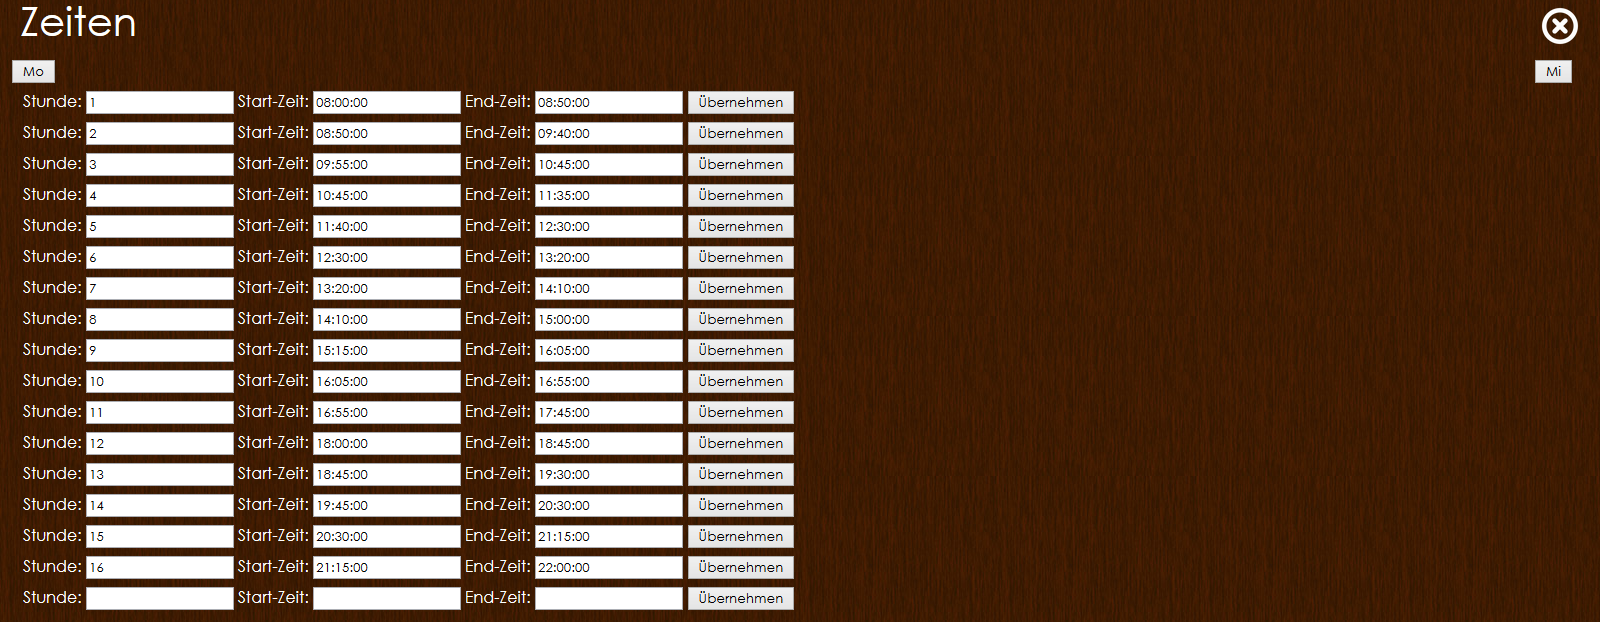
\includegraphics[keepaspectratio=true, width=17cm]{images/screenshots/hours_input.png}
\caption{Stunden bearbeiten}
\label{fig:instr_other_hours}
\end{figure}
\subsection{Stundenpläne}
Stundenpläne werden in dieser Eingabe eingegeben werden. Dazu muss im zuerst erscheinenden Menü die Klasse ausgewählt werden. Der Tag muss nicht ausgewählt werden, wird er nicht ausgewählt, so startet die Eingabe am Montag. Will man jedoch an einem spezifischen Tag die Eingabe beginnen, so muss man das Kürzel des Wochentages eingeben. Zum bestätigen muss auf OK geklickt werden. (Menü siehe \autoref{fig:instr_other_timetables_menu})
\begin{figure}[H]
\centering
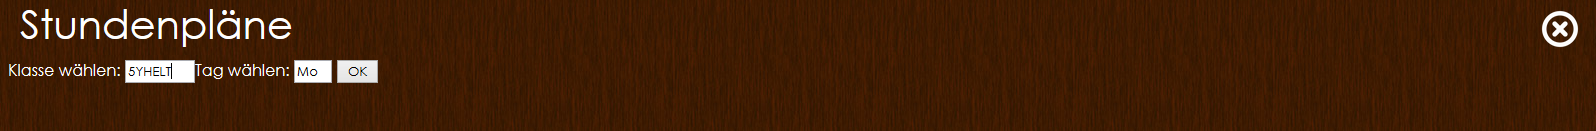
\includegraphics[keepaspectratio=true, width=17cm]{images/screenshots/timetables_input_menu.png}
\caption{Stundenplan auswählen}
\label{fig:instr_other_timetables_menu}
\end{figure}
Ist dies ausgewählt so gelangt man zur Eingabe der gewählten Klasse und des gewählten Tages. Im linken oberen Bereich des Fensters sind die gewählte Klasse und der gewählte Tag zu sehen. Mit einem Klick auf die Klasse gelangt man wieder ins Menü für die Klassenauswahl zurück. (siehe \autoref{fig:instr_other_timetables_infos})
\begin{figure}[H]
\centering
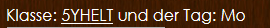
\includegraphics[keepaspectratio=true, width=6cm]{images/screenshots/timetables_input_infos.png}
\caption{Klasse und Tag}
\label{fig:instr_other_timetables_infos}
\end{figure}
Den Tag kann man mit den Buttons, welche links und rechts zu sehen sind, auswählen.  Mit einem Klick auf den Button wechselt man zu dem Tag, der auf dem Button zu sehen ist. (siehe \autoref{fig:instr_other_timetables_infos})
\begin{figure}[H]
\centering
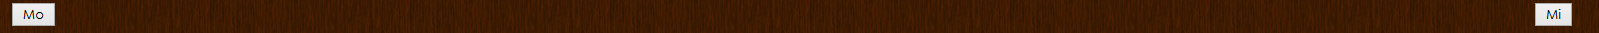
\includegraphics[keepaspectratio=true, width=17cm]{images/screenshots/timetables_input_day.png}
\caption{Tagauswahl}
\label{fig:instr_other_timetables_infos}
\end{figure}
Die Eingabemaske sieht wie in \autoref{fig:instr_other_timetables_layout} zu sehen ist aus. In den nächsten Abschnitten werden verschiedene Eintragungen beschrieben und somit auch die Eingabemaske beschrieben.
\begin{figure}[H]
\centering
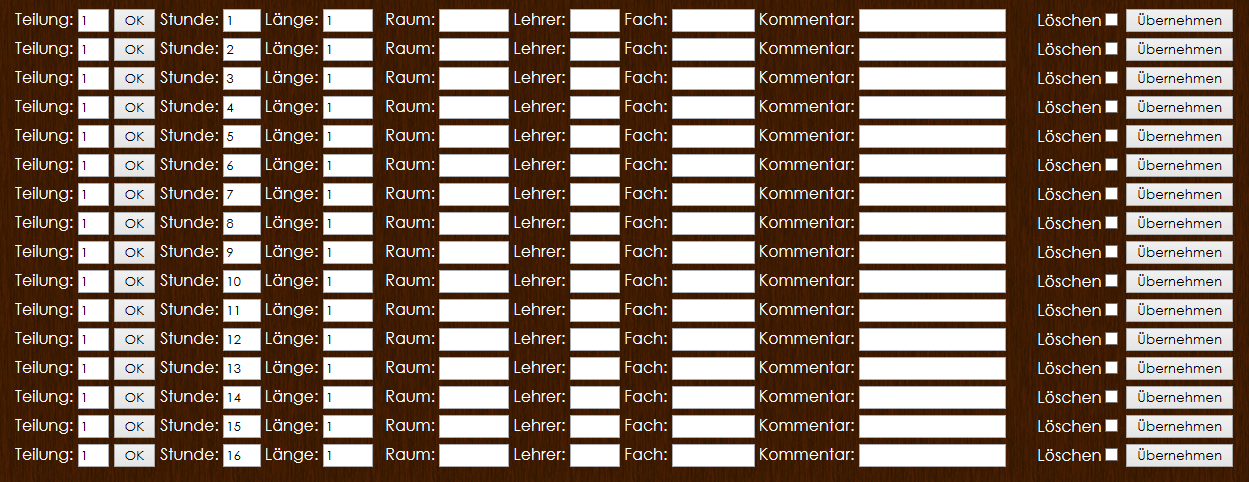
\includegraphics[keepaspectratio=true, width=17cm]{images/screenshots/timetables_input_layout.png}
\caption{Tagauswahl}
\label{fig:instr_other_timetables_layout}
\end{figure}
\subsubsection{Einzelstunde}
Soll eine Stunde eingetragen werden, welche nur eine Stunde lang ist, so muss an der Standardeinstellung nichts geändert werden. Es muss nur das Fach und der Lehrer eingetragen werden. In der zweiten Spalte ist die Stunde zu sehen. Will man in der zweiten Stunde eine Stunde hinzufügen, so muss dort eingetragen werden wo bei der Stunde 2 steht. Hat man die Stunde fertig eingetragen so muss man auf Übernehmen klicken. (Siehe Beispiel in \autoref{fig:instr_other_timetables_singleHour})
\begin{figure}[H]
\centering
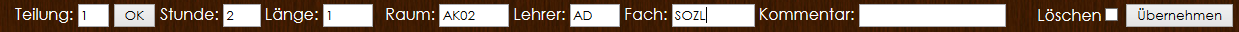
\includegraphics[keepaspectratio=true, width=17cm]{images/screenshots/timetables_input_singleHour.png}
\caption{Beispiel Einzelstunde}
\label{fig:instr_other_timetables_singleHour}
\end{figure}
\subsubsection{Mehrstündige Stunden}
Wenn eine Stunde eingetragen werden soll, die mehr als eine Stunde andauert, so muss dies in der Eingabemaske, dementsprechend vermerkt werden. Dies geschieht in der Textbox Länge. Beginnt die Stunde in der ersten Stunde und dauert 3 Stunden, so muss in der Zeile, in der bei Stunde 1 steht, bei Länge 3 eingefügt werden. Klickt man nun in eine andere Textbox, so werden die Stunden ausgeblendet, die durch die Länge nicht mehr benötigt werden. In diesem Beispiel wird die Stunde 2 und 3 ausgeblendet. Die restlichen eingaben funktionieren nach dem selben Prinzip, wie bei der Einzelstunde. (Siehe Beispiel in \autoref{fig:instr_other_timetables_multiHour})
\begin{figure}[H]
\centering
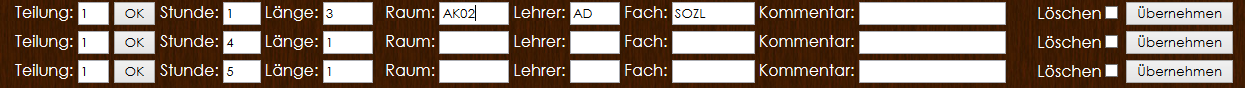
\includegraphics[keepaspectratio=true, width=17cm]{images/screenshots/timetables_input_multiHour.png}
\caption{Beispiel Mehrstündige Stunden}
\label{fig:instr_other_timetables_multiHour}
\end{figure}
\subsubsection{Teilungen}
Da es auch vorkommt, dass eine Klasse in sich geteilt wird, kann auch dies eingegeben werden. Dazu ist die Textbox Teilung zuständig. Dies funktioniert nur wenn die geteilten Fächer genau gleich lang sind. Sind sie unterschiedlich lang, so muss es anders eingegeben werden. Ist die Klasse in sich einmal geteilt und eine Hälfte hat 2 Stunden und die andere Hälfte 3 Stunden Unterricht, so muss die Teilung für die ersten 2 Stunden eingetragen werden und die andere Stunde kann als einzelne Stunde eingetragen werden.\\
Soll nun eine Teilung eingegeben werden, muss zuerst die Anzahl der Teilungen eingegeben werden und anschließend auf OK geklickt werden. Anschließend erscheinen weitere Zeilen. Die maximale Teilung die eingetragen werden kann ist 7 Teilungen. (siehe \autoref{fig:instr_other_timetables_divide7}) Die Länge der Stunde kann gleich wie bei keiner Teilung eingestellt werden.
\begin{figure}[H]
\centering
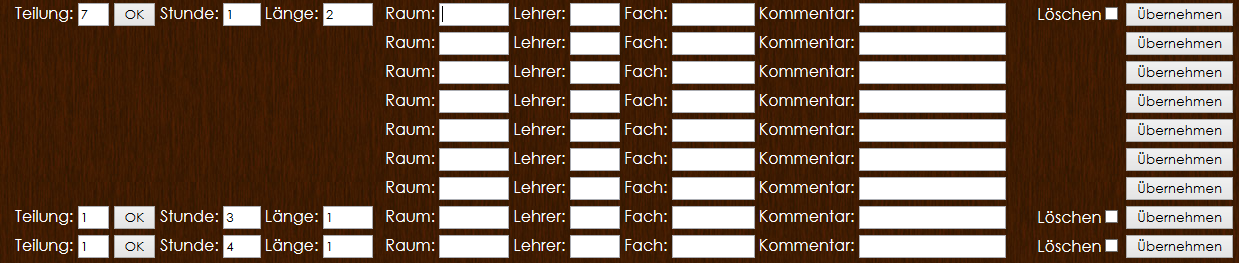
\includegraphics[keepaspectratio=true, width=17cm]{images/screenshots/timetables_input_divide7.png}
\caption{Beispiel Teilungen}
\label{fig:instr_other_timetables_divide7}
\end{figure}
Jede eigene Zeile muss mit Übernehmen bestätigt werden. Gelöscht kann jedoch nur ein ganzer Block werden. Dies muss mit einem Hacken bei Löschen und anschließendem klicken auf Übernehmen erfolgen.
\subsubsection{Löschen}
Es können prinzipiell ganze Stundenblöcke gelöscht werden, jedoch gibt es noch die Möglichkeit den ganzen Tag dieser Klasse zu löschen. Dies geschieht mit dem Button links oben. (siehe \autoref{fig:instr_other_timetables_delete}) Klickt man auf diesen Button werden die Stunden dieser Klasse und dieses Tages unwiderruflich gelöscht.
\begin{figure}[H]
\centering
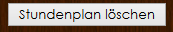
\includegraphics[keepaspectratio=true, width=5cm]{images/screenshots/timetables_input_delete.png}
\caption{Löschen}
\label{fig:instr_other_timetables_delete}
\end{figure}
\subsection{Lehrer}
Dieser Punkt ist dazu da, dass man Lehrer bearbeiten und hinzufügen kann. Auch hier ist es nicht möglich Lehrer zu löschen, da es wie bei Stunden zu großen Problemen kommen kann. (siehe \autoref{sec:instr_other_hidden})\\
Im Feld Name muss der vollständige Name des Lehrers eingegeben werden, im Feld Kürzel wird das Lehrer-Kürzel eingetragen, im Feld Kurzname muss ein verkürzter Name eingegeben werden, dieser wird zum Beispiel bei den Supplierungen am Display angezeigt. Im Feld Stammabteilung kann eine Abteilung eingegeben werden, dies ist jedoch optional, da nicht jeder Lehrer eine Stammabteilung hat. Wie schon erwähnt ist der Hacken für unsichtbar zum stilllegen eines Lehrers gut. (Eingabemaske siehe \autoref{fig:instr_other_teacher}) Sollen vorhandene Daten geädert werden, so kann man den vorhandenen Lehrer abändern un mit Übernehmen speichern.
\begin{figure}[H]
\centering
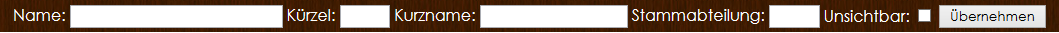
\includegraphics[keepaspectratio=true, width=17cm]{images/screenshots/teachers_input.png}
\caption{Eingabemaske Lehrer}
\label{fig:instr_other_teacher}
\end{figure}
\subsection{Fächer}
Müssen Fächer abgeändert oder hinzugefügt werden, so ist dies mit diesem Punkt möglich. Hier gilt wieder, das Fach kann nur unsichtbar gemacht werden. (siehe \autoref{sec:instr_other_hidden})\\
Im Feld Name wird der vollständige Name des Faches eingetragen, im Feld Kürzel wird die Kurzbezeichnung des Faches eingegeben, welche in den Stundenpläne, Supplierpläne und so weiter sichtbar sind. Die Eingabe kann jeweils mit Übernehmen gesichert werden. Wie bei allen Eingabemasken können auch vorhandene Einträge bearbeitet werden, die abgeänderte Daten müssen mit übernehmen gesichert werden. (Eingabemaske siehe \autoref{fig:instr_other_subjects})
\begin{figure}[H]
\centering
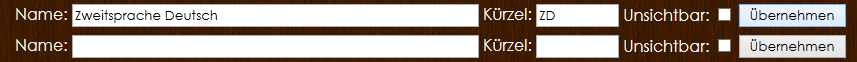
\includegraphics[keepaspectratio=true, width=17cm]{images/screenshots/subjects_input.png}
\caption{Eingabemaske Fächer}
\label{fig:instr_other_subjects}
\end{figure}
\subsection{Statistiken}
Um die Nutzung und um zu sehen, ob unser Service auch bei den Nutzern angenommen wird, haben wir uns beschlossen außerhalb des vorgegeben Pflichtenheftes eine Statistik anzulegen. Im Folgendem werden die einzelnen Diagramme beschrieben. Wichtig ist, dass wir, das Entwicklerteam ausgenommen sind, da dies die ganze Statistik verfälschen würde.\\
Im linken oberen Bereich können die Statistiken mit einem Klick auf Reload neu geladen werden. (siehe \autoref{fig:instr_other_statistics_header})
\begin{figure}[H]
\centering
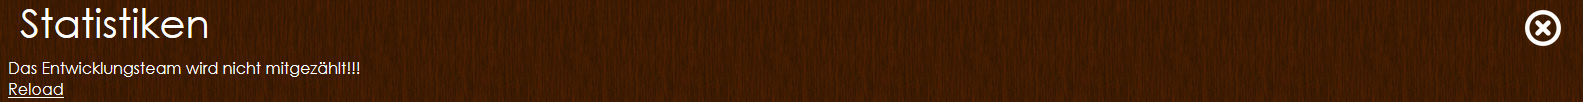
\includegraphics[keepaspectratio=true, width=17cm]{images/screenshots/statistics_header.png}
\caption{Statistiken Reload}
\label{fig:instr_other_statistics_header}
\end{figure}
\subsubsection{Browser PC}
In dieser Statistik sind die Browser der Geräte dargestellt, welche die PC Seiten aufrufen. (siehe \autoref{fig:instr_other_statistics_browser_PC})
\begin{figure}[H]
\centering
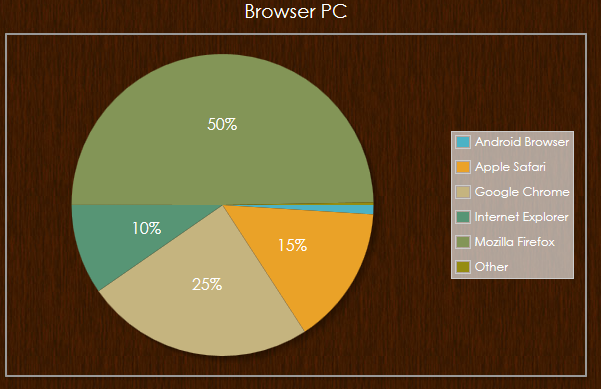
\includegraphics[keepaspectratio=true, width=8cm]{images/screenshots/statistics_browser_PC.png}
\caption{Browser PC}
\label{fig:instr_other_statistics_browser_PC}
\end{figure}
\subsubsection{Geräte PC}
In dieser Statistik sind die Geräte bzw. Betriebssysteme der Geräte dargestellt, welche die PC Seiten aufrufen. (siehe \autoref{fig:instr_other_statistics_os_PC})
\begin{figure}[H]
\centering
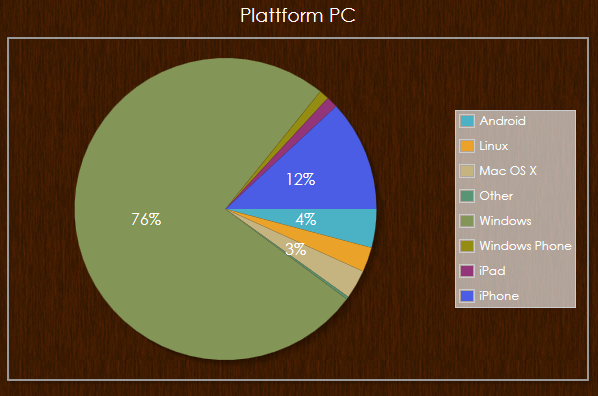
\includegraphics[keepaspectratio=true, width=8cm]{images/screenshots/statistics_os_PC.png}
\caption{Geräte PC}
\label{fig:instr_other_statistics_os_PC}
\end{figure}
\subsubsection{Browser Mobil}
In dieser Statistik sind die Browser der Geräte dargestellt, welche die App aufrufen. (siehe \autoref{fig:instr_other_statistics_browser_Mob})
\begin{figure}[H]
\centering
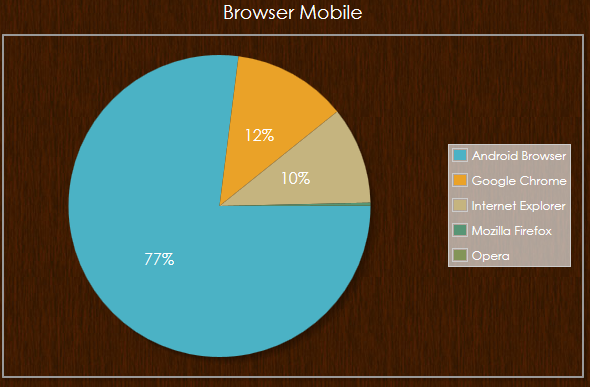
\includegraphics[keepaspectratio=true, width=8cm]{images/screenshots/statistics_browser_Mob.png}
\caption{Browser Mobil}
\label{fig:instr_other_statistics_browser_Mob}
\end{figure}
\subsubsection{Geräte Mobil}
In dieser Statistik sind die Geräte bzw. Betriebssysteme der Geräte dargestellt, welche die App Seiten aufrufen. (siehe \autoref{fig:instr_other_statistics_os_Mob})
\begin{figure}[H]
\centering
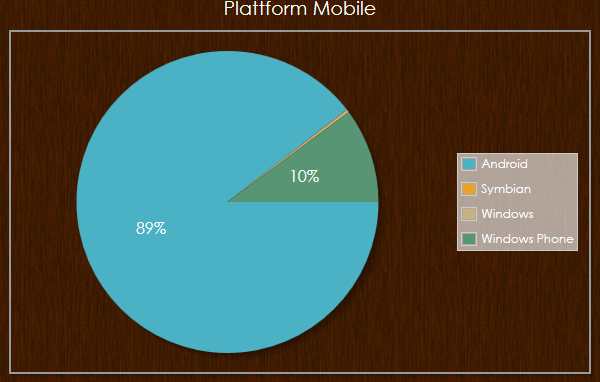
\includegraphics[keepaspectratio=true, width=8cm]{images/screenshots/statistics_os_Mob.png}
\caption{Browser PC}
\label{fig:instr_other_statistics_os_Mob}
\end{figure}
\subsubsection{Nutzer}
In dieser Statistik sind die Nutzer nach den Schulstufen und nach den Lehrern aufgeteilt. Hier kann herausgelesen werden welcher Jahrgang den Service am häufigsten nutzt. (siehe \autoref{fig:instr_other_statistics_user})
\begin{figure}[H]
\centering
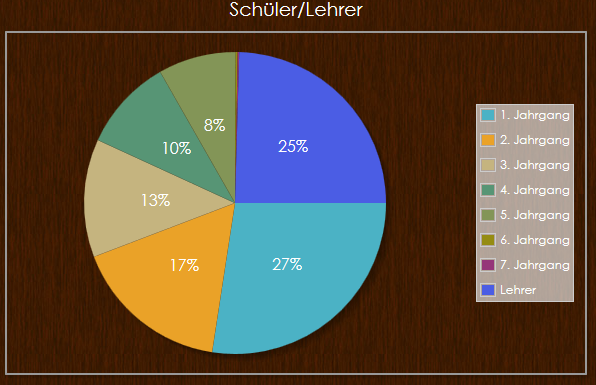
\includegraphics[keepaspectratio=true, width=8cm]{images/screenshots/statistics_user.png}
\caption{Nutzer}
\label{fig:instr_other_statistics_user}
\end{figure}
\subsubsection{Abteilungen}
In dieser Statistik werden die Nutzer nach ihrer Abteilung aufgeteilt, dabei werden nur die Schüler gezählt. Hier kann herausgelesen werden welche Abteilung den Service am häufigsten nutzt. (siehe \autoref{fig:instr_other_statistics_sections})
\begin{figure}[H]
\centering
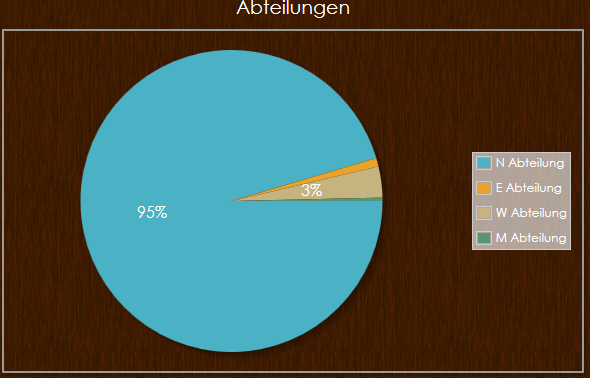
\includegraphics[keepaspectratio=true, width=8cm]{images/screenshots/statistics_sections.png}
\caption{Abteilungen}
\label{fig:instr_other_statistics_sections}
\end{figure}
\subsubsection{Supplierunen}
In dieser Statistik wird dargestellt welche Seite die User am häufigsten benützen, um die Supplierungen anzusehen. Dabei wird der Supplierplan im Web, Supplierplan in der App , der modifizierte Stundenplan in der App und der modifizierte Stundenplan im Web analysiert. (siehe \autoref{fig:instr_other_statistics_substitudes})
\begin{figure}[H]
\centering
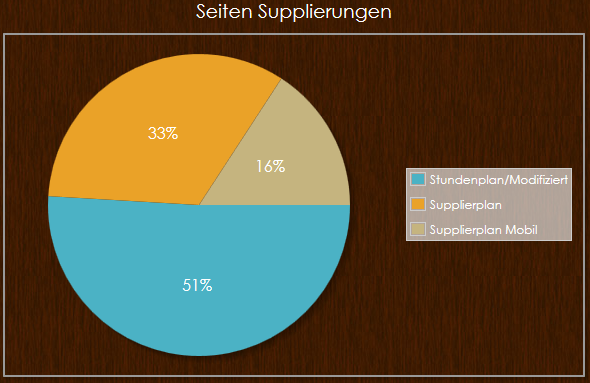
\includegraphics[keepaspectratio=true, width=8cm]{images/screenshots/statistics_substitudes.png}
\caption{Supplierungen}
\label{fig:instr_other_statistics_substitudes}
\end{figure}
\subsubsection{App/Web}
In dieser Statistik wird die App und die Webseite gegenübergestellt und man kann auslesen welcher Dienst öfters genutzt wird. (siehe \autoref{fig:instr_other_statistics_app_web})
\begin{figure}[H]
\centering
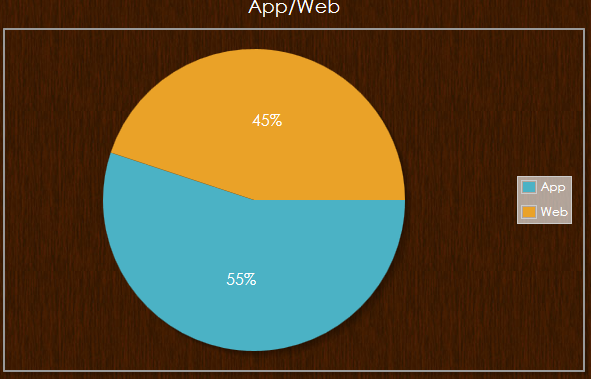
\includegraphics[keepaspectratio=true, width=8cm]{images/screenshots/statistics_app_web.png}
\caption{App/Web}
\label{fig:instr_other_statistics_app_web}
\end{figure}
\subsubsection{Seiten Web}
In dieser Statistik wird dargestellt welche Seiten die User auf der Webseite am häufigsten besuchen. (siehe \autoref{fig:instr_other_statistics_sites_web})
\begin{figure}[H]
\centering
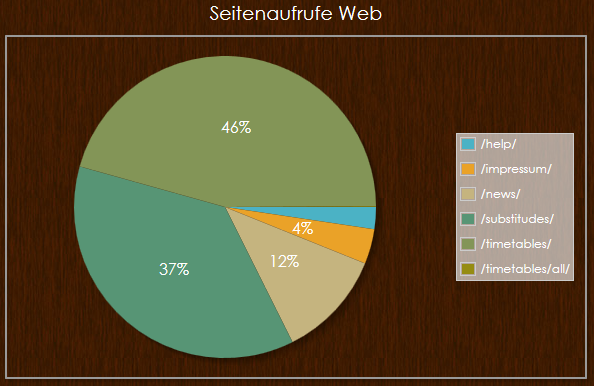
\includegraphics[keepaspectratio=true, width=8cm]{images/screenshots/statistics_sites_web.png}
\caption{Seiten Web}
\label{fig:instr_other_statistics_sites_web}
\end{figure}
\subsubsection{Seiten App}
In dieser Statistik wird dargestellt welche Seiten die User in der App am häufigsten besuchen. (siehe \autoref{fig:instr_other_statistics_sites_app})
\begin{figure}[H]
\centering
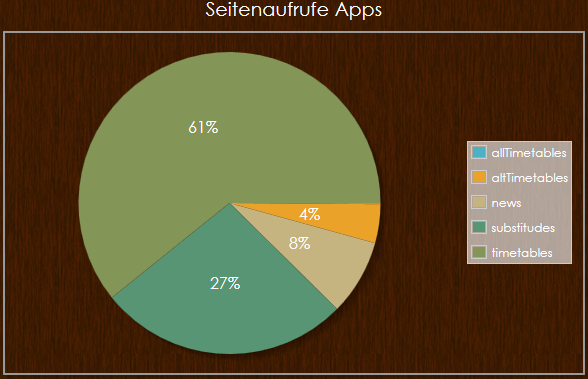
\includegraphics[keepaspectratio=true, width=8cm]{images/screenshots/statistics_sites_app.png}
\caption{Seiten App}
\label{fig:instr_other_statistics_sites_app}
\end{figure}
\subsubsection{Seitenaufrufe Stunden}
In dieser Statistik wird dargestellt, wie viele Seitenaufrufe im Durchschnitt in welcher Stunde am Tag auftreten. (siehe \autoref{fig:instr_other_statistics_view_day})
\begin{figure}[H]
\centering
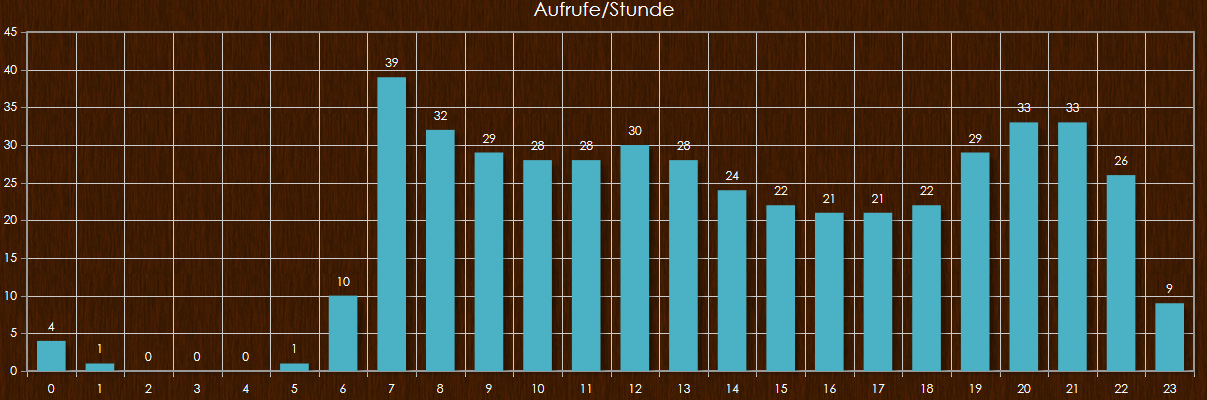
\includegraphics[keepaspectratio=true, width=17cm]{images/screenshots/statistics_views_hour.png}
\caption{Seitenaufrufe Stunden}
\label{fig:instr_other_statistics_view_day}
\end{figure}
\subsubsection{Seitenaufrufe täglich}
In dieser Statistik wird dargestellt, wie viele Seitenaufrufe jeden Tag verursacht werden. (siehe \autoref{fig:instr_other_statistics_views_day}) Hier kann auch, um bei vielen Tagen den Überblick zu beschaffen, in die Tage hineingezoomt werden. Dies macht man in dem man mit der rechten Maustaste ein gewünschtes Fenster aufzieht. Heraus zoomen kann mit einem doppelten rechts Klick gemacht werden. (siehe \autoref{fig:instr_other_statistics_views_day_zoom})
\begin{figure}[H]
\centering
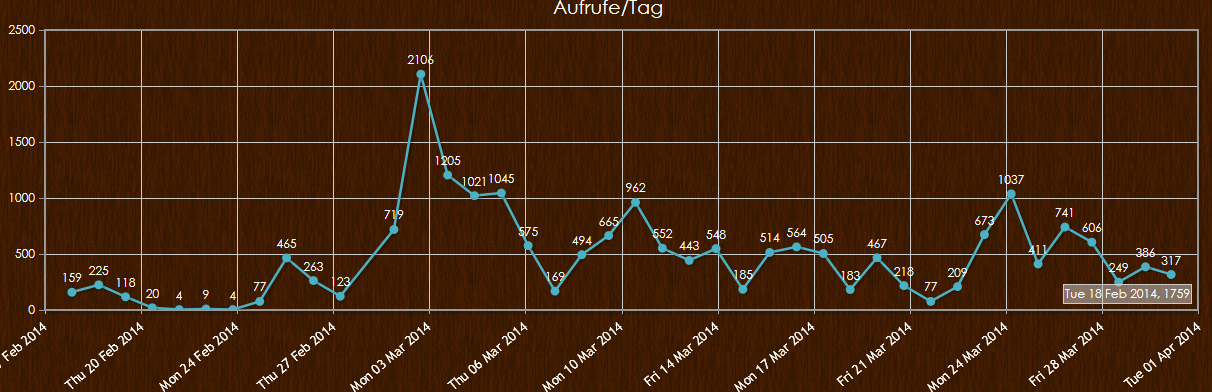
\includegraphics[keepaspectratio=true, width=17cm]{images/screenshots/statistics_views_day.png}
\caption{Seitenaufrufe täglich}
\label{fig:instr_other_statistics_views_day}
\end{figure}
\begin{figure}[H]
\centering
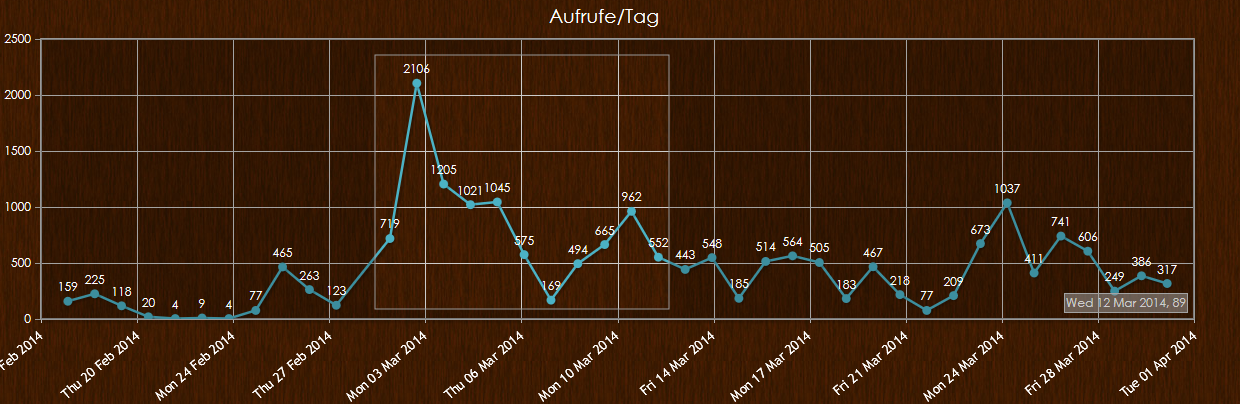
\includegraphics[keepaspectratio=true, width=17cm]{images/screenshots/statistics_views_day_zoom.png}
\caption{Seitenaufrufe täglich zoomen}
\label{fig:instr_other_statistics_views_day_zoom}
\end{figure}
\subsection{Räume}
Sollen neue Räume hinzugefügt werden oder bestehende geändert werden, dann kann dies in dieser Eingabe vorgenommen werden. Der unterschied zu den anderen Eingaben ist, dass man Räume nicht löschen oder unsichtbar machen kann, da ein Raum üblicherweise nicht entfernt wird. Sollte es jedoch doch einmal zu einem Fall kommen, dass ein Raum entfernt werden soll, so kann dies nicht gemacht werden. Dieser Raum scheint trotzdem in der Liste auf.\\
Im Feld Name wird der Raumname eingetragen und im Feld zuständiger Lehrer kann ein für diesen Raum verantwortlicher Lehrer eingetragen werden, dieses Feld ist jedoch optional und muss nicht verwendet werden. Mit Übernehmen werden die Daten gespeichert. (Eingabemaske siehe \autoref{fig:instr_other_room_input})
\begin{figure}[H]
\centering
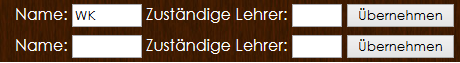
\includegraphics[keepaspectratio=true, width=10cm]{images/screenshots/rooms_input.png}
\caption{Eingabemaske Räume}
\label{fig:instr_other_room_input}
\end{figure}
\subsection{Klassen}
Sollen Klassen verändert oder neue hinzugefügt werden, so kann dies in dieser Eingabemaske vorgenommen werden. Klassen können auch nicht gelöscht werden, jedoch können diese unsichtbar gemacht werden. (siehe \autoref{sec:instr_other_hidden}) Da es vorkommen kann dass in einem Jahr eine Klasse nicht gibt, aber im nächsten Jahr.\\
Im ersten Feld Name kann der Name der Klasse eingegeben werden, im Feld Abteilung wird der Klasse eine Abteilung zugewiesen, im Feld Klassenvorstand wird der Klasse ein Klassenvorstand zugewiesen. Hat die Klasse eine Stammklasse kann auch diese angegeben werden. Als Scheinklasse können den Wanderklassen der Raum WK zugewiesen werden, jedoch ist dieses Feld optional und muss nicht angegeben werden. Das Klassenvorstand Feld ist ebenfalls optional. (Eingabemaske siehe \autoref{fig:instr_other_classes_input})
\begin{figure}[H]
\centering
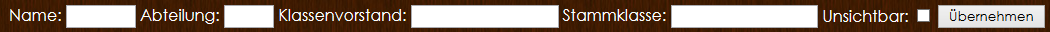
\includegraphics[keepaspectratio=true, width=17cm]{images/screenshots/classes_input.png}
\caption{Eingabemaske Klassen}
\label{fig:instr_other_classes_input}
\end{figure}
\subsection{Abteilungen}
Kommt es vor, dass sich ein Name einer Abteilung ändert oder es kommt eine neue Abteilung hinzu, so kann dies in dieser Eingabe vorgenommen werden. Abteilungen können weder gelöscht noch unsichtbar gemacht werden. (siehe \autoref{sec:instr_other_hidden})\\
Im ersten Feld Name wird der Name der Abteilung eingegeben, im Feld Kürzel wird das Kürzel der Abteilung eingegeben und im Feld Abteilungsvorstand wird der Abteilungsvorstand eingegeben. Mit Übernehmen müssen die Daten gespeichert werden. (Eingabemaske siehe \autoref{fig:instr_other_sections_input})
\begin{figure}[H]
\centering
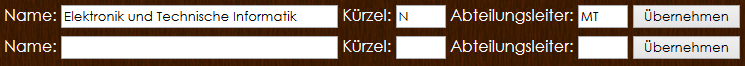
\includegraphics[keepaspectratio=true, width=17cm]{images/screenshots/sections_input.png}
\caption{Eingabemaske Abteilungen}
\label{fig:instr_other_sections_input}
\end{figure}
\subsection{Unsichtbar}\label{sec:instr_other_hidden}
Aus Sicherheitsgründen können manche Daten nicht gelöscht werden, da es bei unabsichtlichem Löschen dazu kommt, dass andere Daten nicht mehr vollständig sind und deshalb das ganze System zusammenbrechen kann.\\
Deshalb gibt es in manchen Eingaben keine Lösch-Funktion, in manchen gibt es jedoch eine Unsichtbar-Funktion. Mit dieser Funktion werden die Daten in der Eingabe ganz nach unten gereiht und werden in den DropDown Menüs nicht mehr angezeigt.\\
Unsichtbar gemachte Daten können auch wieder reaktiviert werden.
\subsection{DropDown-Menüs}
In den meisten Eingaben sind den Textfeldern Daten hinterlegt, welche bei beginn mit dem eintippen schon die möglichen Daten anzeigt. wird bei Ende der Eingabe kein Vorschlag angezeigt so kann man davon ausgehen, dass der Eingegebene Wert nicht vorhanden ist. Diese Funktion ist jedoch nicht bei jedem Textfeld verfügbar.